%!TEX root = ../thesis.tex

\chapter{Підготовка до розробки}
\label{chap:review}  %% відмічайте кожен розділ певною міткою -- на неї наприкінці необхідно посилатись

Для початку нам знадобиться криптовалютний web3-гаманець для подальшого розгортання та демонстрування роботи смарт-контракту. В нашому випадку ми скористаємося найбільш популярним таким гаманцем -- Metamask, який використовується для взаємодії з блокчейном Ethereum. Для роботи з ним потрібно встановити та налаштувати Metamask у вашому браузері. \par
Більш детальна інструкція доступна за посиланням: \\ \url{https://support.metamask.io/getting-started/getting-started-with-metamask/}. \par
Далі наведемо основні кроки.

\section{Як встановити MetaMask}

\begin{enumerate}
    \item Відвідайте \url{https://metamask.io/}.
    
    \begin{figure}[ht]
        \centering
        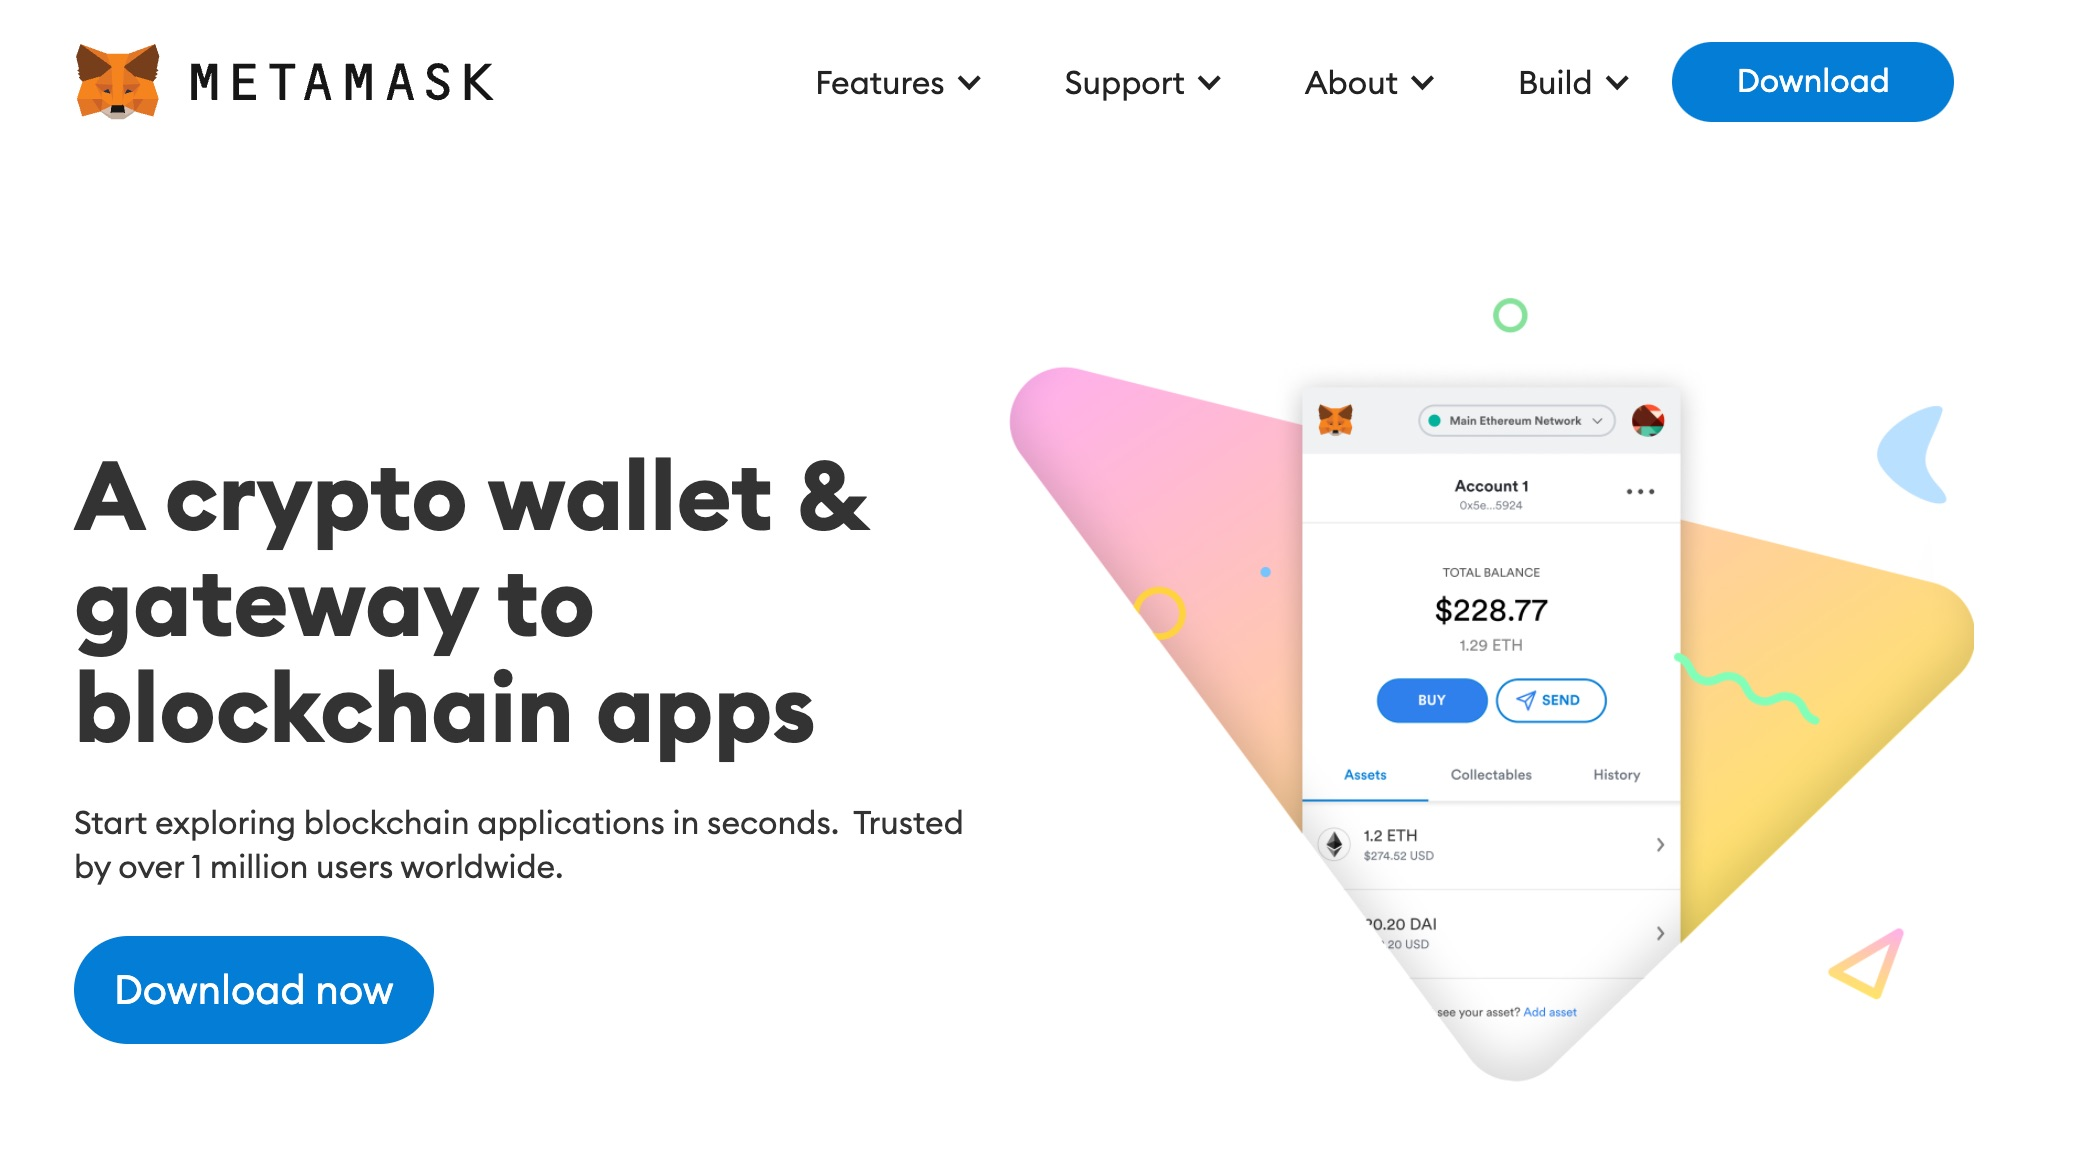
\includegraphics[scale=0.22]{IMAGES/metamask1.jpeg}
        \caption{Сайт metamask.io.}
        \label{fig_sudak}
    \end{figure}
    
    \item Натисніть «Завантажити» на панелі меню.

    \item Натисніть «Встановити MetaMask для Chrome». Вас буде спрямовано до веб-магазину Chrome.

    \begin{figure}[ht]
        \centering
        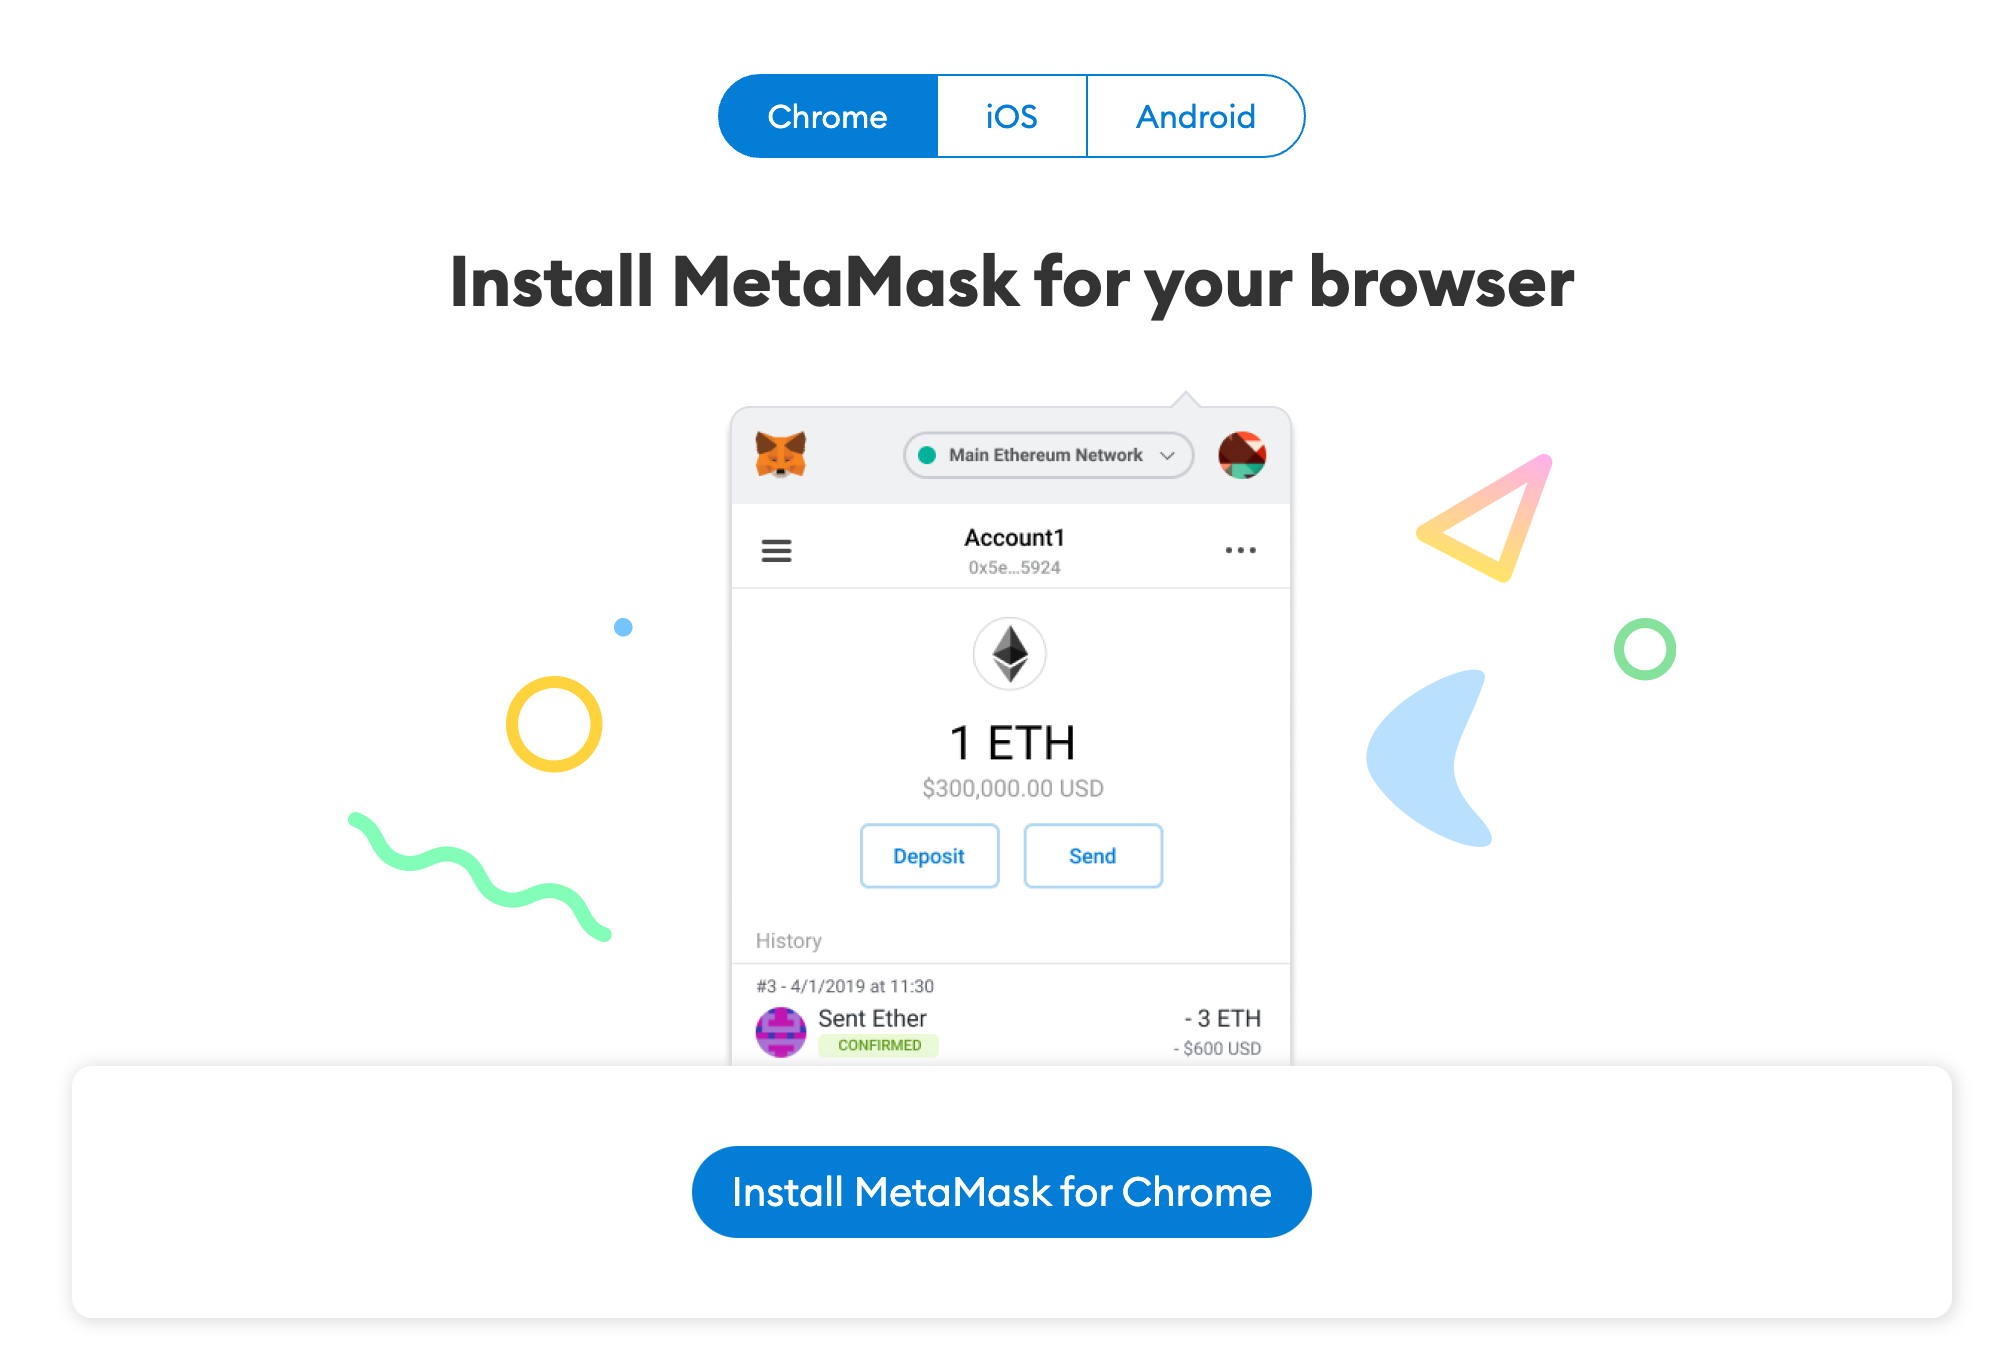
\includegraphics[scale=0.45]{IMAGES/metamask2.png}
        \caption{Вибір методу встановлення MetaMask-гаманця.}
        \label{fig_sudak}
    \end{figure}

    \item Натисніть «Додати в Chrome».

    \begin{figure}[ht]
        \centering
        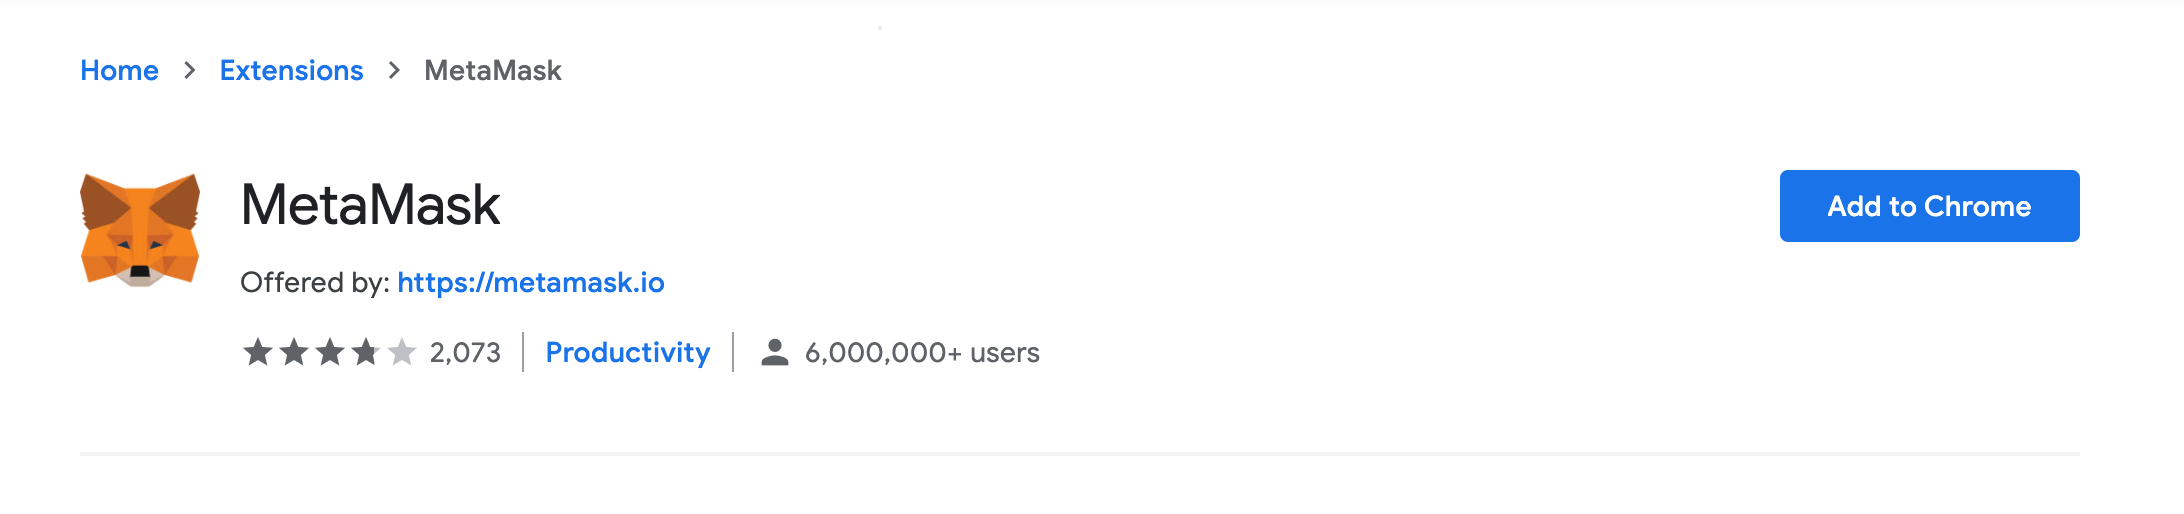
\includegraphics[scale=0.4]{IMAGES/metamask3.png}
        \caption{Встановлення розширення MetaMask для Chrome.}
        \label{fig_sudak}
    \end{figure}

    \newpage
    \item У спливаючому вікні натисніть «Додати розширення».
    
    \begin{figure}[ht]
            \centering
            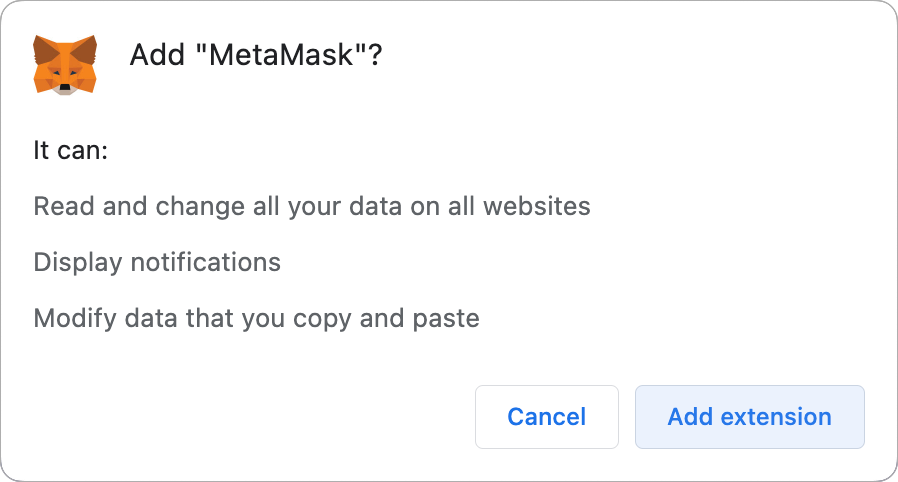
\includegraphics[scale=0.5]{IMAGES/metamask4.png}
            \caption{Спливаюче вікно «Додати розширення».}
            \label{fig_pacman}
    \end{figure}

    Після додавання розширення MetaMask відкриється автоматично. Ви також можете переконатися, що він легко доступний на панелі інструментів, клацнувши піктограму головоломки у верхньому правому куті екрана та натиснувши піктограму шпильки.  

    \begin{figure}[ht]
            \centering
            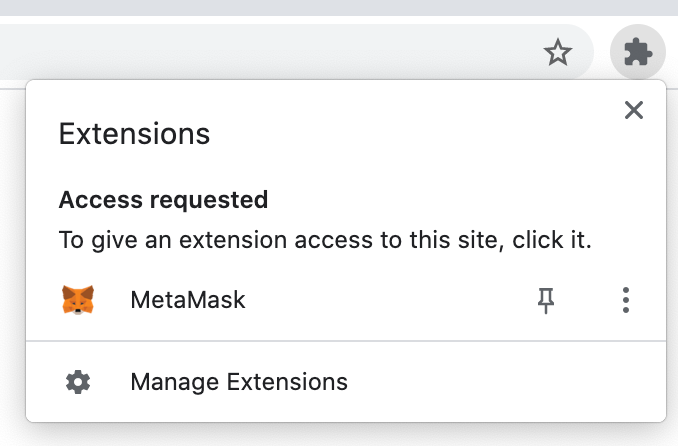
\includegraphics[scale=0.5]{IMAGES/metamask5.png}
            \caption{MetaMask на панелі інструментів.}
            \label{fig_pacman}
    \end{figure}

    Після того, як ви закріпите розширення, ви побачите його тут у верхньому правому куті веб-переглядача.

     \begin{figure}[ht]
            \centering
            
\includegraphics[scale=0.5]{IMAGES/metamask6.png}
            \caption{MetaMask у верхньому куті веб-переглядача.}
            \label{fig_pacman}
    \end{figure}

\end{enumerate}

\section{Як налаштувати MetaMask}

\begin{enumerate}

\item Після встановлення вас повинно перенаправити до такої сторінки.

    \begin{figure}[ht]
            \centering
            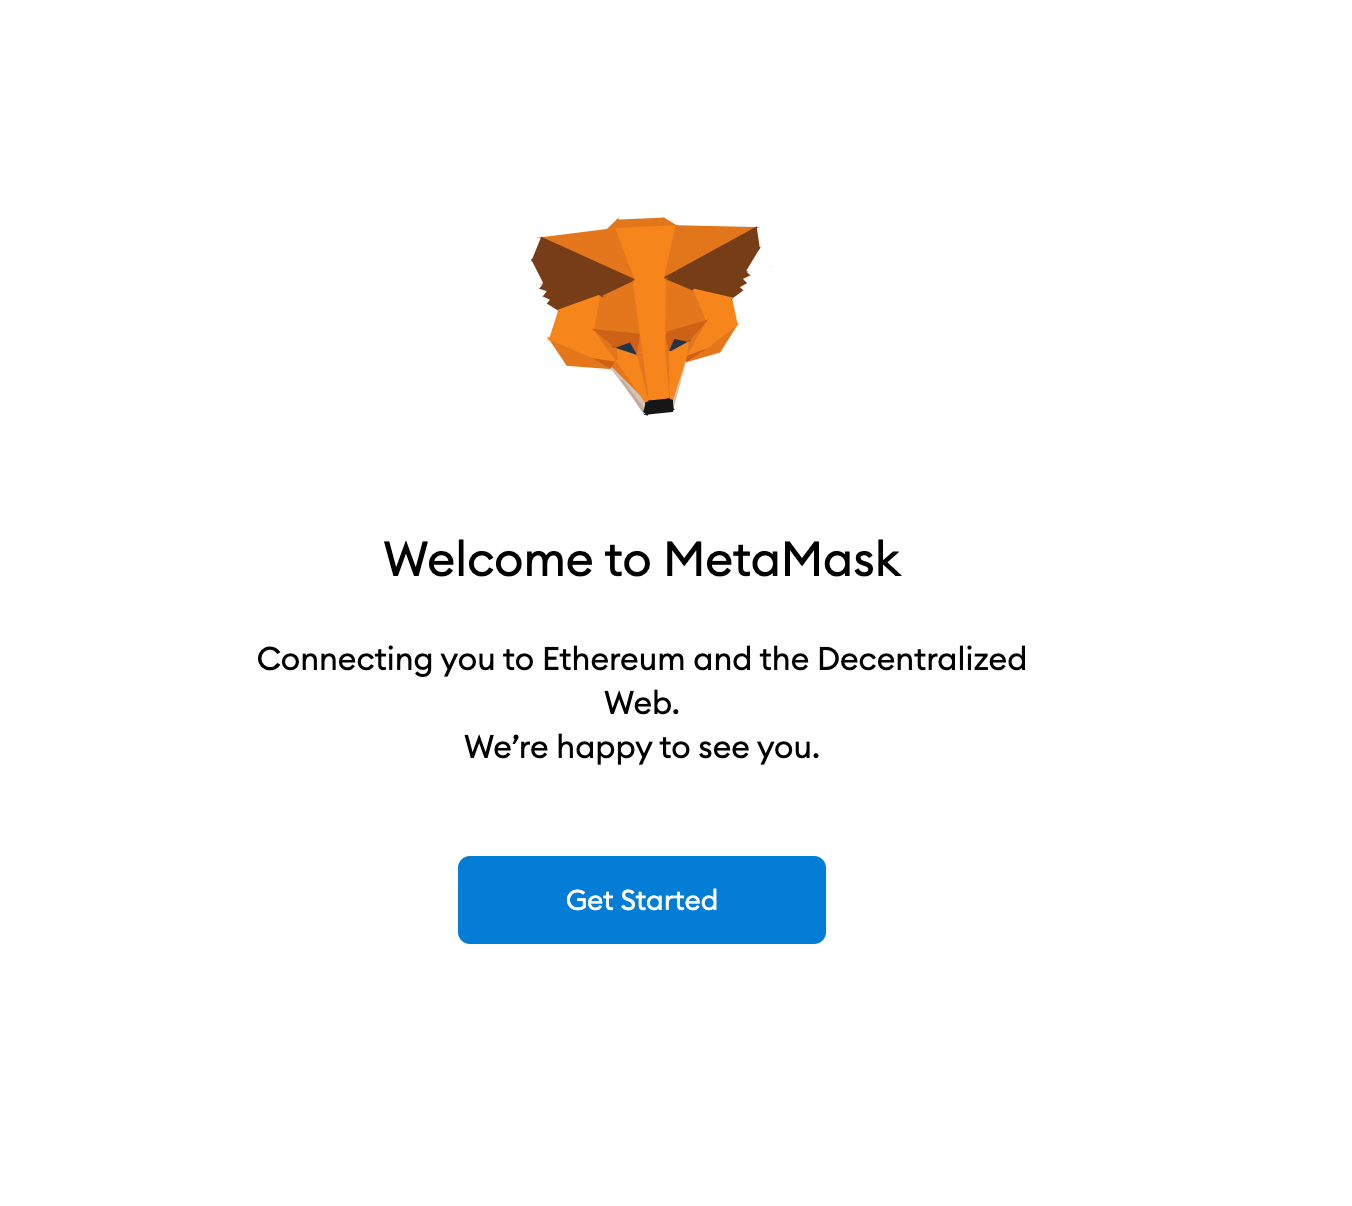
\includegraphics[scale=0.4]{IMAGES/metamask7.png}
            \caption{Початкова сторінка MetaMask.}
            \label{fig_pacman}
    \end{figure}

\item Тепер, коли ви встановили MetaMask, у вас є розширення для браузера. Потім ви потрапите на сторінку, яка виглядає так. Оскільки це ми вперше, ми виберемо «Створити гаманець».

    \begin{figure}[ht]
            \centering
            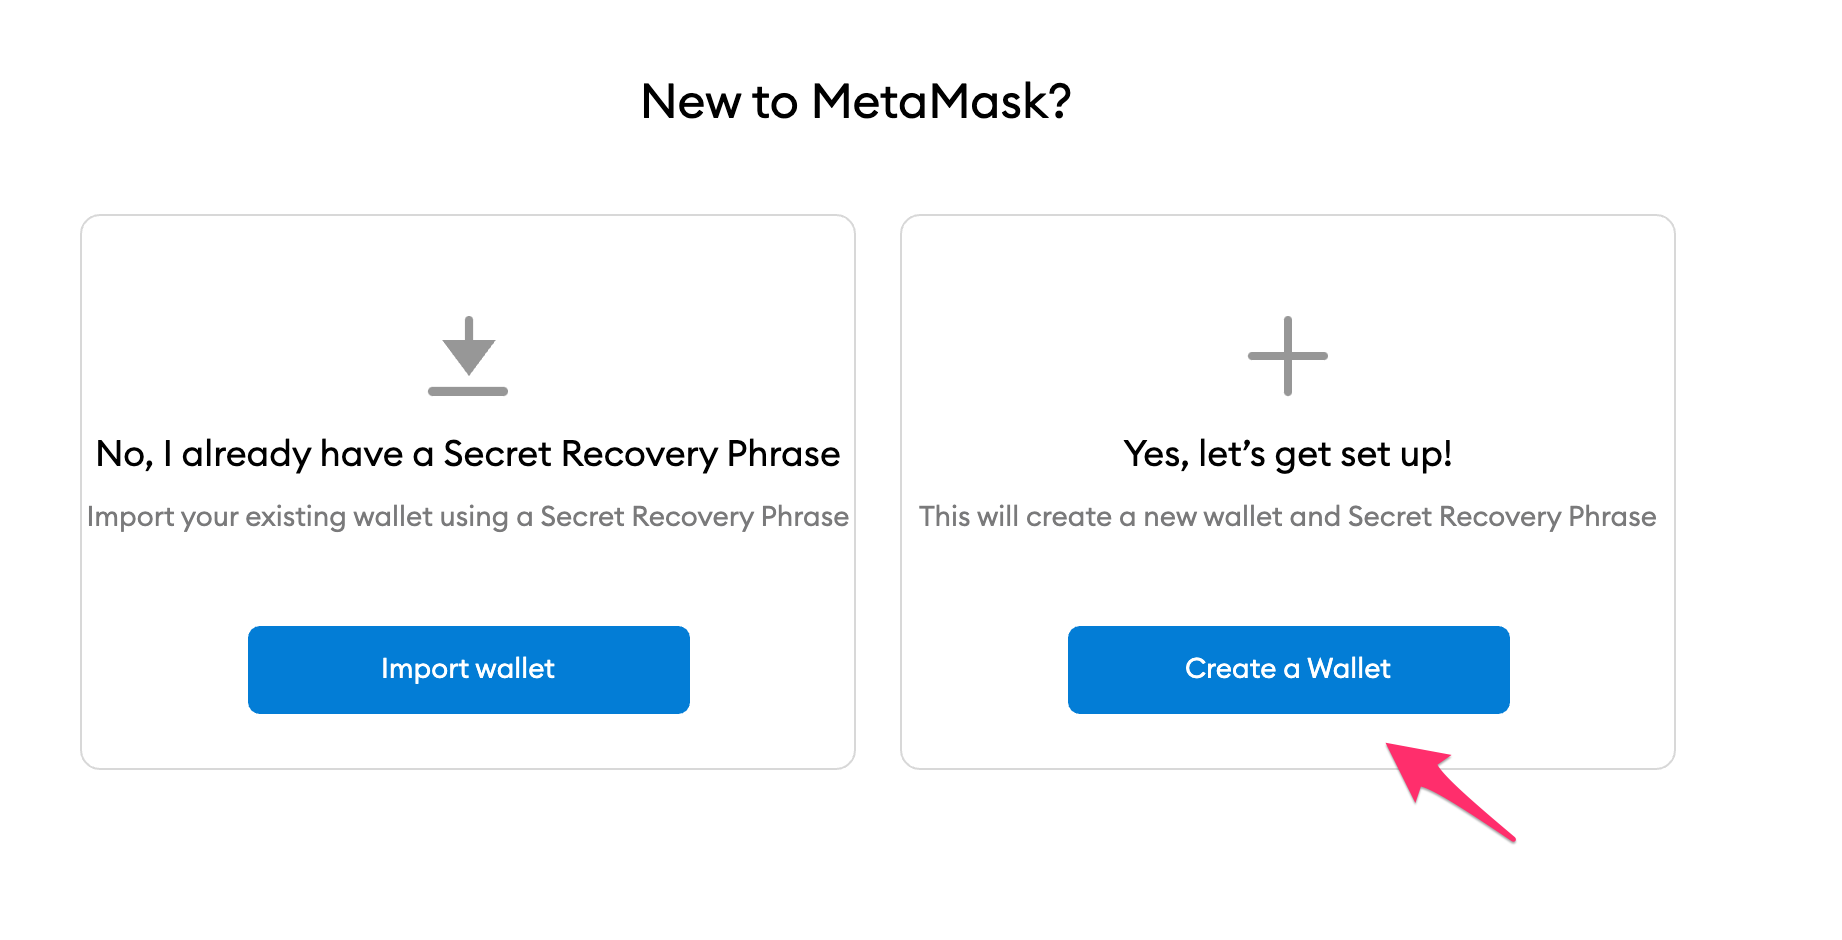
\includegraphics[scale=0.4]{IMAGES/metamask8.png}
            \caption{Сторінка <<Створити гаманець>>.}
            \label{fig_pacman}
    \end{figure}

\item Тепер ви створюєте пароль. Це розблокує розширення MetaMask на вашому комп’ютері. Введіть свій пароль і натисніть «Створити».

\item Далі вам буде запропоновано резервну фразу Secrete. Це також може мати інші назви, як-от фраза відновлення або фраза гаманця. Це ваш суперсекретний пароль, який надає доступ до вашого гаманця.

Якщо ви втратите цю фразу, ви втратите доступ до своїх жетонів. Якщо хтось інший отримає цю фразу, він отримає доступ до вашого гаманця.

Натисніть, щоб відкрити секретні слова. Це фраза з 12 слів.

    \begin{figure}[ht]
            \centering
            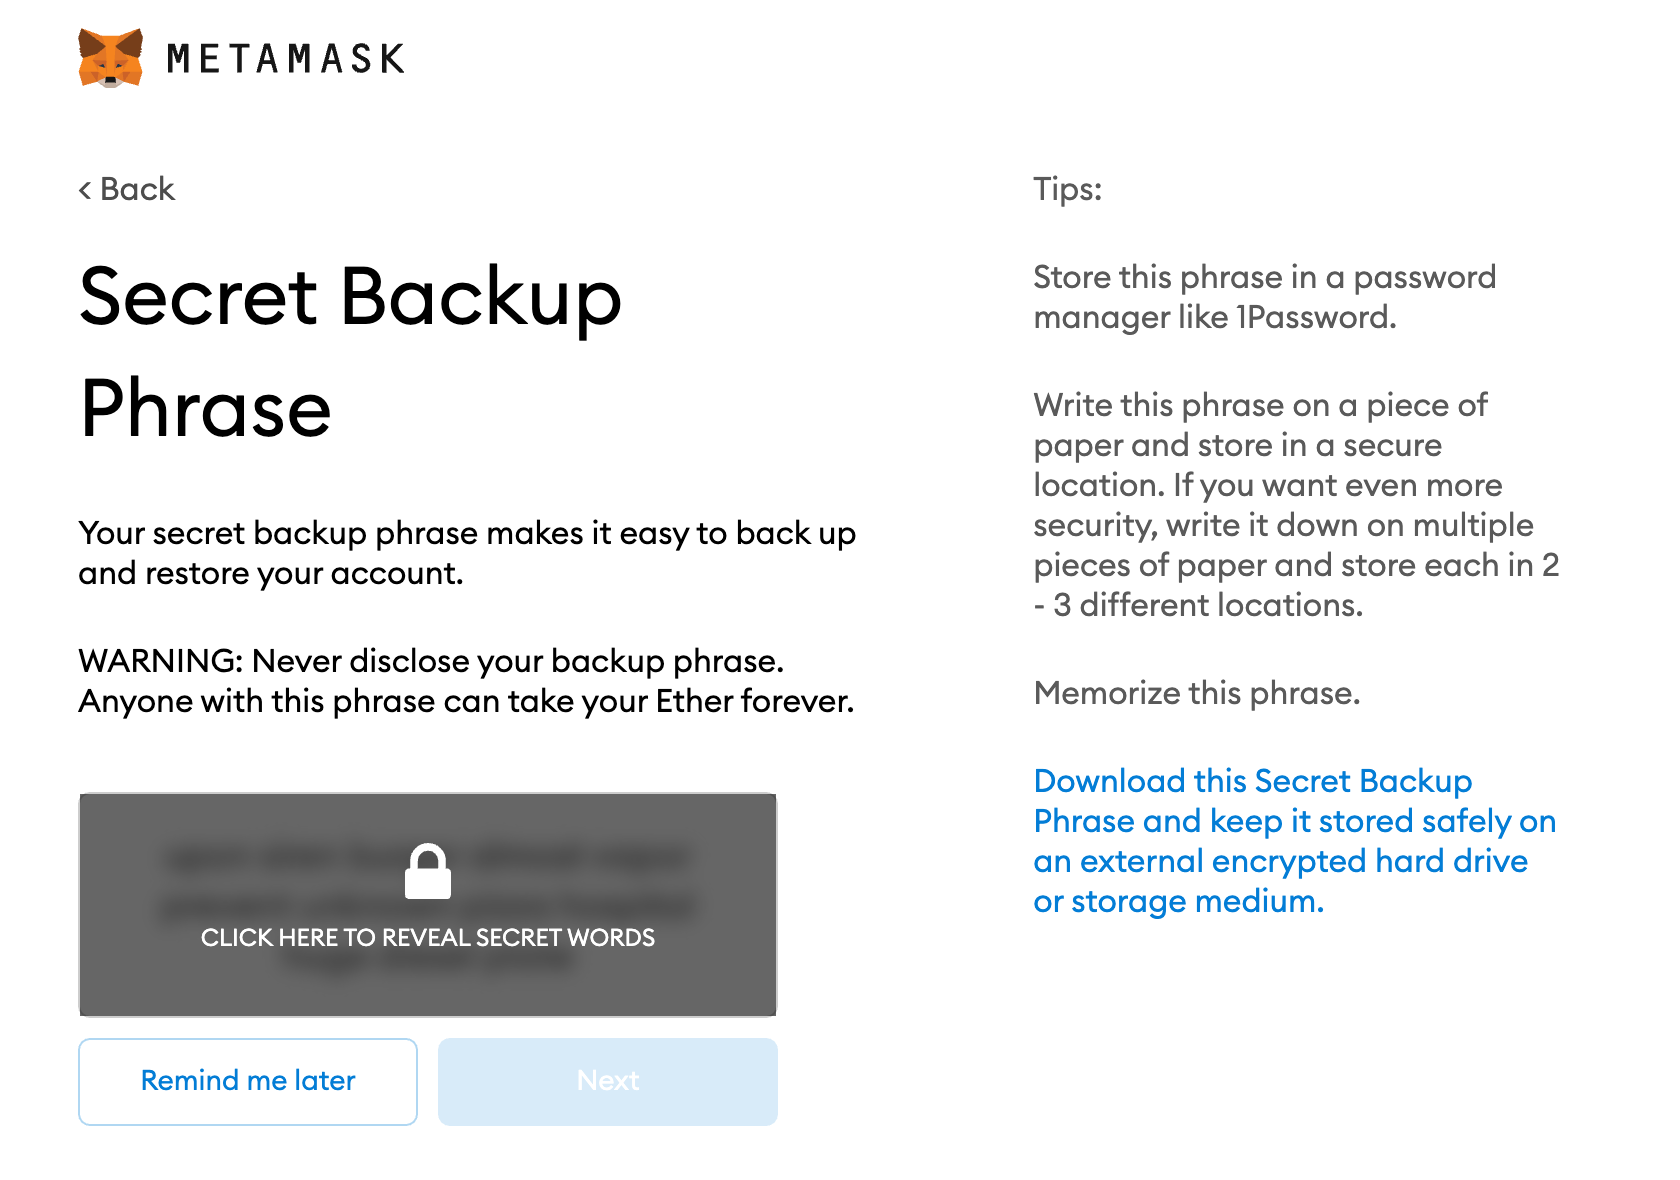
\includegraphics[scale=0.5]{IMAGES/metamask9.png}
            \caption{Сторінка <<Secret Backup Phrase>>.}
            \label{fig_pacman}
    \end{figure}

\item Тепер, коли ви налаштували свій гаманець, ви можете знайти свою адресу Ethereum. Ви можете відкрити свій гаманець, натиснувши значок лисиці у верхньому правому куті, і це відкриє ваш гаманець. Тепер, якщо ви клацнете літери та цифри, які починаються з "0x...", і скопіюєте це - це ваша адреса.

    \begin{figure}[ht]
            \centering
            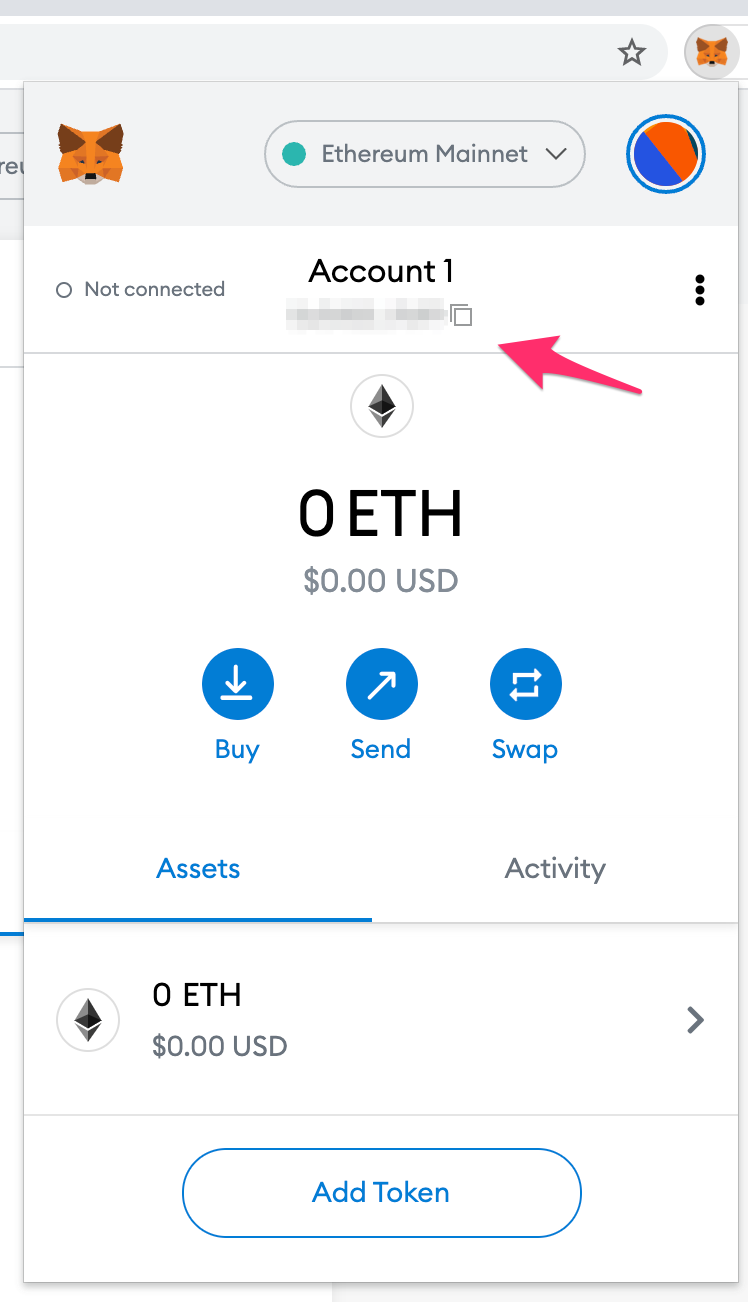
\includegraphics[scale=0.4]{IMAGES/metamask10.png}
            \caption{Адреса вашого MetaMask-гаманця.}
            \label{fig_pacman}
    \end{figure}
    
\newpage
Ви також можете натиснути три крапки, щоб переглянути «Деталі облікового запису», або натиснути «Переглянути на Etherscan».

\end{enumerate}

\section{Тестова мережа Ethereum -- Sepolia}

Ми плануємо розгорнути власний смарт-контракт в тестовій мережі Sepolia, тому нам знадобиться певна кількість криптовалюти для погашення комісій. Одним зі способів безкоштовного отримання невеликої, але достатньої кількості криптовалюти для нашого завдання є так звані криптокрани.

Криптокрани --- це платформи, які надають користувачам невелику кількість криптовалюти за виконання простих завдань. Девіз цих платформ <<Отримайте безкоштовні тестові ETH прямо на свій гаманець>>.

Ми ж будемо користуватися одним з найбільш популярних таких криптокранів -- Sepolia Faucet від Alchemy. Alchemy пропонує крановий сервіс для тестових мереж Ethereum Goerli та Sepolia. Alchemy переказує до 0,5 Sepolia ETH щодня. Для того, щоб запобігти зловживанням, для доступу до сервісу faucet необхідний обліковий запис Alchemy.

\begin{enumerate}
    \item Спочатку створіть обліковий запис Alchemy, щоб запросити Sepolia ETH за посиланням: \href{https://auth.alchemy.com/signup?redirectUrl=https%3A%2F%2Fdashboard.alchemy.com%2Fsignup%3Fa%3Dsepolia_faucet%26redirectUrl%3Dhttps%253A%252F%252Fsepoliafaucet.com%252F%253FauthRefresh%253DTrue}{https://auth.alchemy.com/signup/}.
    
    \begin{figure}[ht]
            \centering
            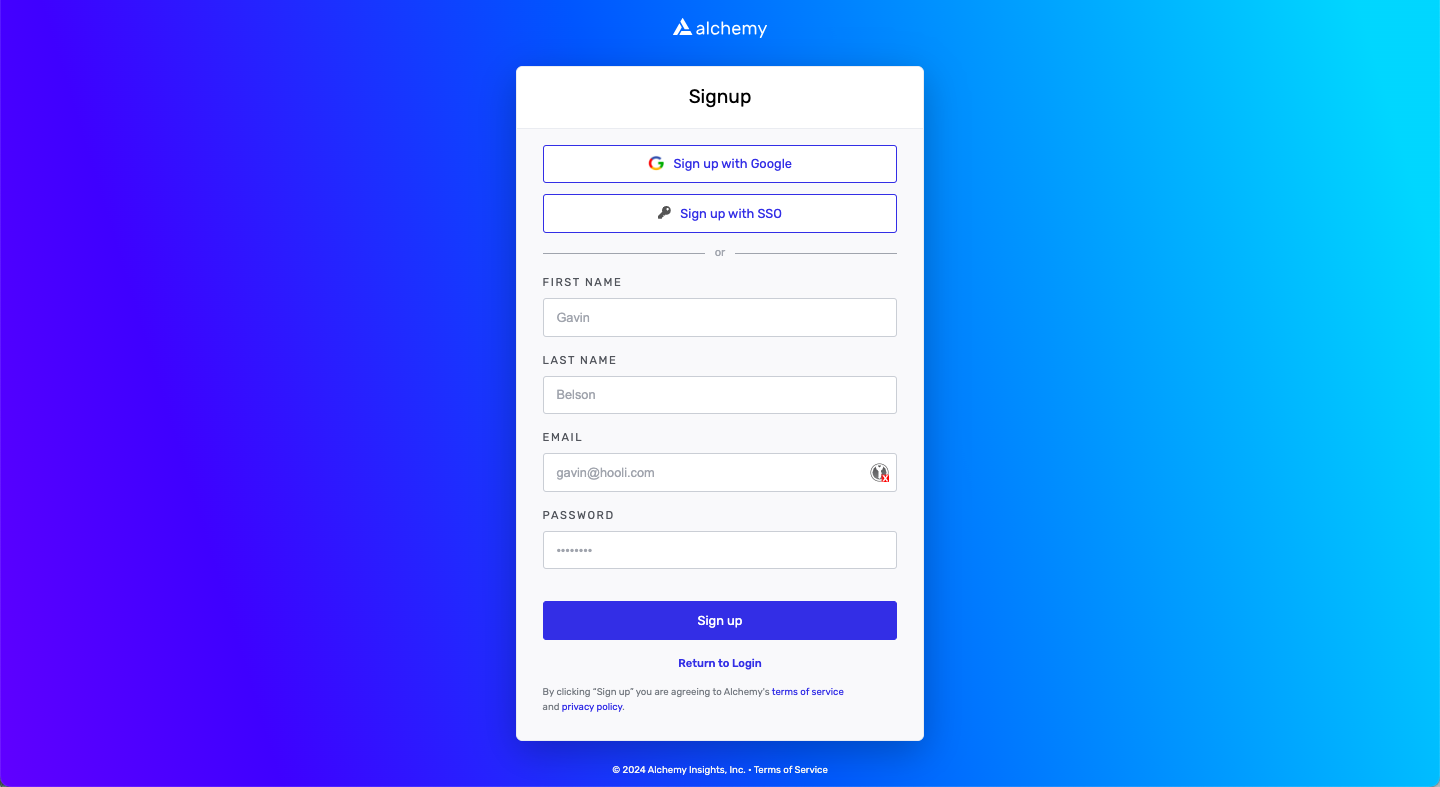
\includegraphics[scale=0.25]{IMAGES/metamask11.png}
            \caption{Вікно реєстрації Alchemy.}
            \label{fig_pacman}
    \end{figure}

    \item Відвідайте криптокран Alchemy Sepolia за посиланням \url{https://www.alchemy.com/faucets/base-sepolia} та увійдіть за допомогою свого облікового запису Alchemy.

    \item Введіть свій гаманець у відповідне поле, пройдіть перевірку CAPTCHA і натисніть "Надіслати мені ETH".

    \begin{figure}[ht]
            \centering
            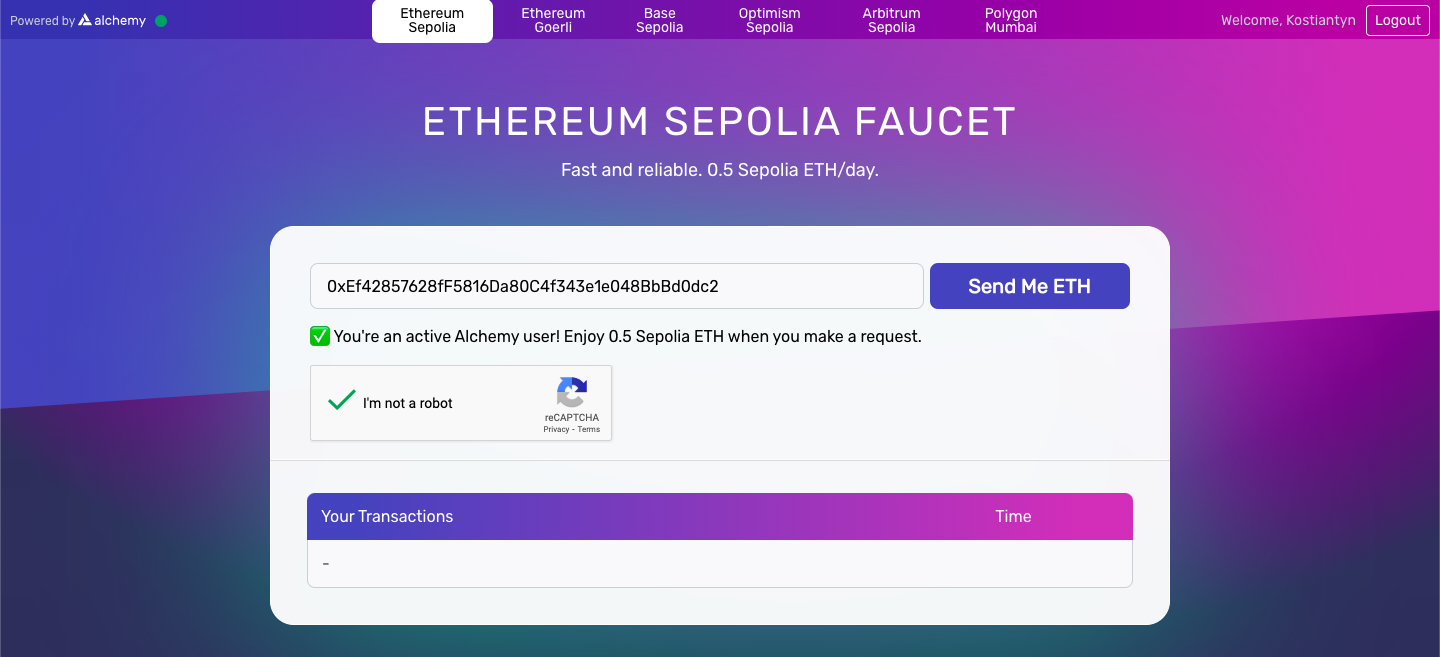
\includegraphics[scale=0.3]{IMAGES/metamask12.png}
            \caption{Вікно введення адреси гаманця для отримання ETH.}
            \label{fig_pacman}
    \end{figure}

    Sepolia ETH будуть відправлені на ваш гаманець і будуть доступні після завершення транзакції. 
    
    Після успішного завершення транзакції ви побачите наступне:

    \begin{figure}[ht]
            \centering
            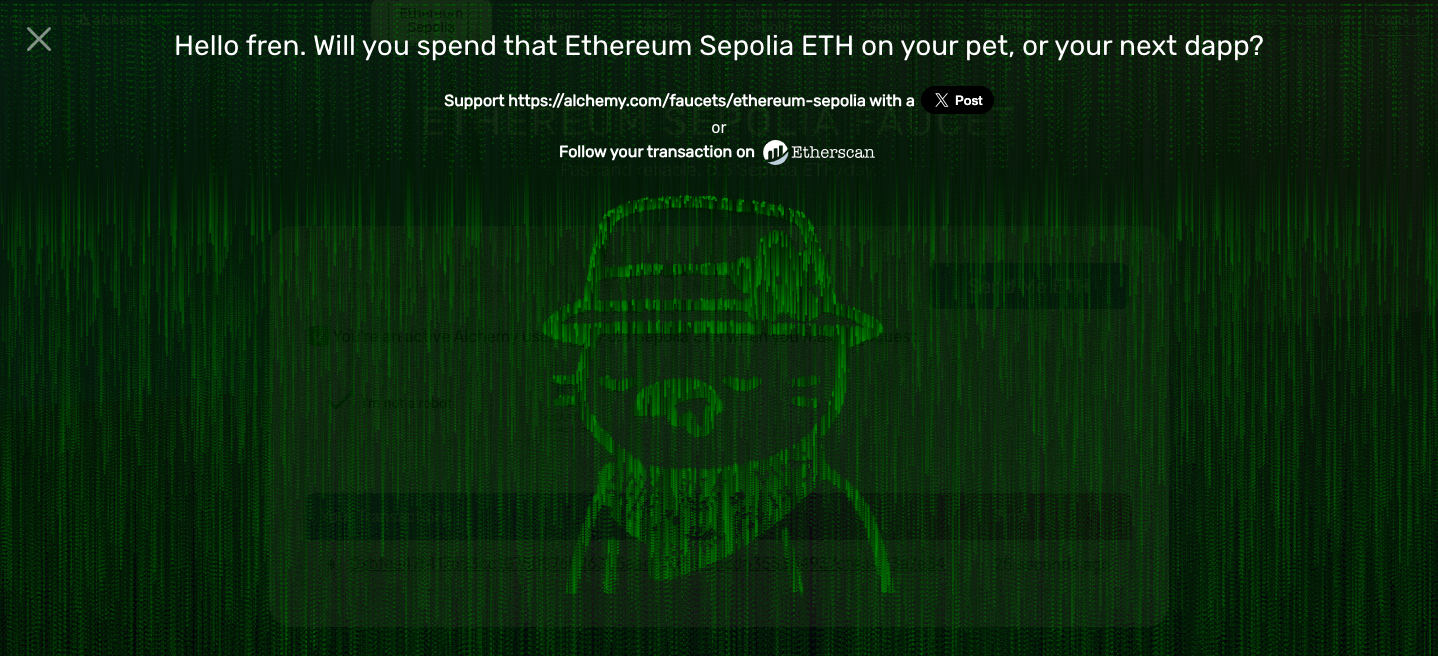
\includegraphics[scale=0.3]{IMAGES/metamask13.png}
            \caption{Вікно успішного завершення транзакції.}
            \label{fig_pacman}
    \end{figure}

    Тепер для того, щоб мати змогу використувати отримані ETH в тестовій мережі Sepolia, вам необхідно змінити у вашому гаманці мережу на Sepolia.
    
    \item Відкрийте MetaMask і натисніть на випадаюче меню вгорі ліворуч:

    \begin{figure}[ht]
            \centering
            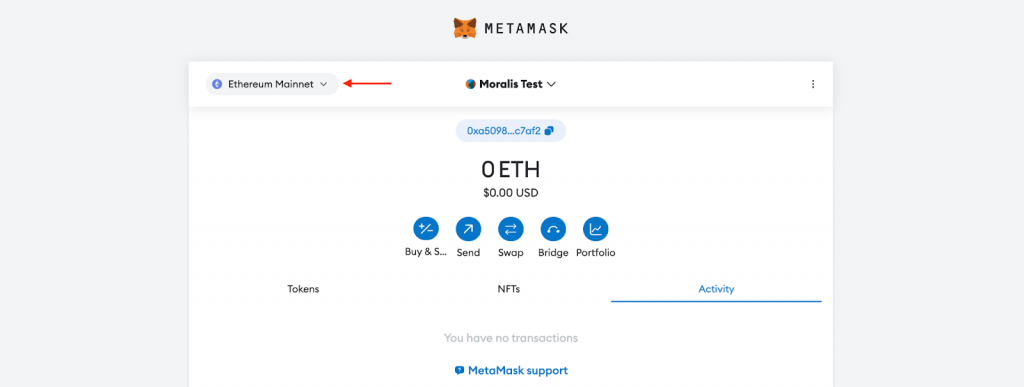
\includegraphics[scale=0.6]{IMAGES/metamask14.png}
            \caption{Зміна мережі в гаманці MetaMask.}
            \label{fig_pacman}
    \end{figure}

    \newpage
    \item Далі ввімкніть кнопку "Показати тестові мережі":

    \begin{figure}[ht]
            \centering
            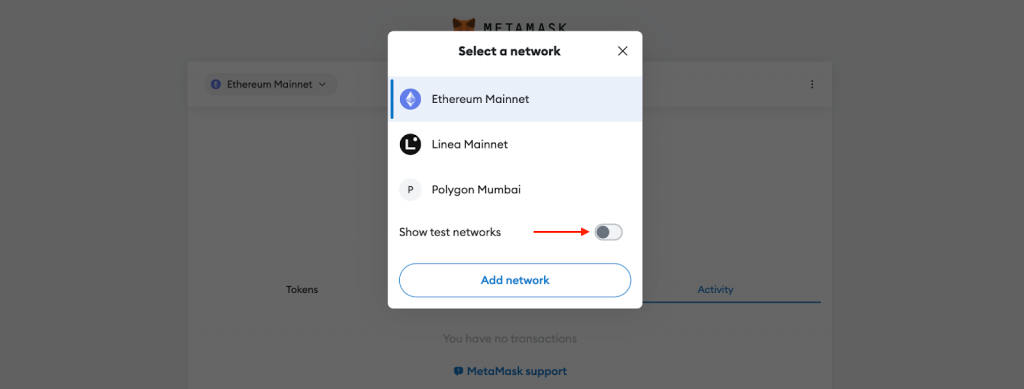
\includegraphics[scale=0.6]{IMAGES/metamask15.png}
            \caption{Зміна мережі в гаманці MetaMask.}
            \label{fig_pacman}
    \end{figure}

    \item Нарешті, натисніть на альтернативу "Sepolia", щоб змінити мережу MetaMask:

    \begin{figure}[ht]
            \centering
            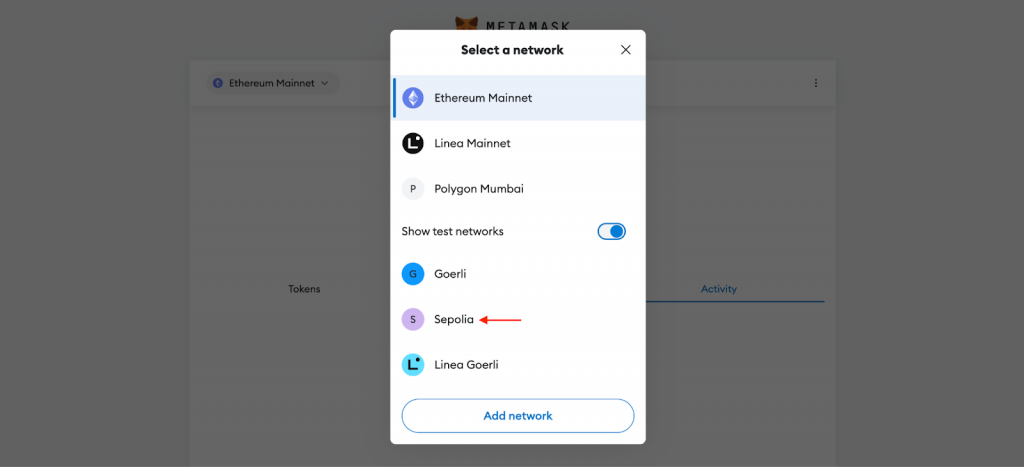
\includegraphics[scale=0.6]{IMAGES/metamask16.png}
            \caption{Зміна мережі в гаманці MetaMask.}
            \label{fig_pacman}
    \end{figure}

    \newpage
    \item Ось і все; тепер ви переключити вашу мережу MetaMask з основної мережі Ethereum на мережу Sepolia:

    \begin{figure}[ht]
            \centering
            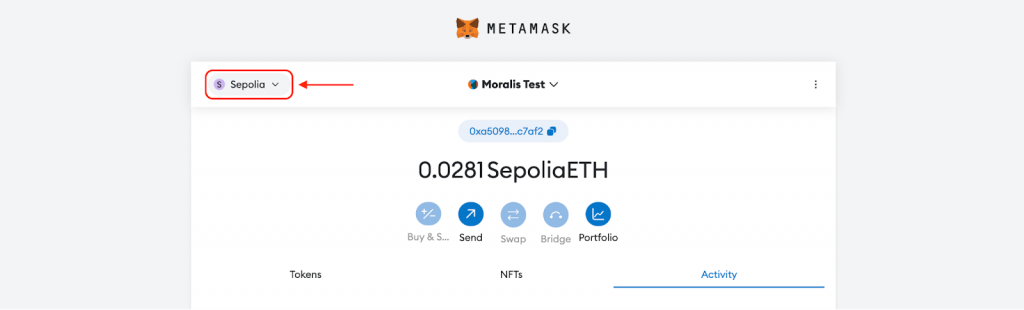
\includegraphics[scale=0.6]{IMAGES/metamask17.png}
            \caption{Зміна мережі в гаманці MetaMask.}
            \label{fig_pacman}
    \end{figure}
    
\end{enumerate}

Тепер перейдемо до розділу безпосередньо розробки власного смарт-контракту та його розгортання в тестовій мережі Sepolia.

% \chapconclude{\ref{chap:review}}

% Наприкінці кожного розділу ви повинні навести коротенькі підсумки по його 
% результатах. Зокрема, для оглядового розділу в якості висновків необхідно 
% зазначити, які задачі у даній тематиці вже були розв'язані, а саме 
% поставлена вами задача розв'язана не була (або розв'язана погано), тому у 
% наступних розділах ви її й розв'язуєте.

% Якщо ваш звіт складається з одного розділу, пропускайте висновок до 
% нього~-- він повністю включається в загальні висновки до роботи